\documentclass{standalone}
\usepackage{tikz}
\begin{document}
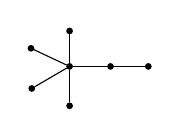
\begin{tikzpicture}[every node/.style={draw, circle, fill=black, minimum size=2pt, inner sep=0pt}]
\node[fill=black] (G1N2) at (6.01,5.22) {};
\node[fill=black] (G1N0) at (6.49,5.50) {};
\node[fill=black] (G1N1) at (7.01,5.50) {};
\node[fill=black] (G1N6) at (7.49,5.50) {};
\node[fill=black] (G1N3) at (6.00,5.73) {};
\node[fill=black] (G1N4) at (6.49,5.00) {};
\node[fill=black] (G1N5) at (6.49,5.95) {};
\draw (G1N0) -- (G1N1);
\draw (G1N0) -- (G1N2);
\draw (G1N0) -- (G1N3);
\draw (G1N0) -- (G1N4);
\draw (G1N0) -- (G1N5);
\draw (G1N1) -- (G1N6);
\end{tikzpicture}
\end{document}
